\scanpage{32}
\[
Q^{2\nu}:\quad \xi:\ H^{2i}(\deleted{\unsure{\xi_2|\xi_\nu}}Q^{2\nu})
\text{---}H^{2i+2}(\deleted{\unsure{\xi_2|\xi_\nu}}Q^{2\nu})(1)
\]
\deleted{\uline{injectif} si $\unsure{2i<2\nu}$ i.e. $i\leq\nu-1$}
    
\uline{bijectif} si $i\neq\nu-1,\nu$
\margin{\deleted{$\unsure{i\geq0}$} ($0\leq i\leq2\nu-1$)}

$i=\nu-1$ : \uline{injectif} \deleted{si $i=\unsure{\nu+1}$}, conoyau libre de base $\unsure{\varphi_\nu|\alpha_\nu}$

$i=\nu$\qquad \deleted{\unsure{surjectif}}\inserted{\uline{surjectif}}, noyau libre de base $\lambda_\nu$

\figure{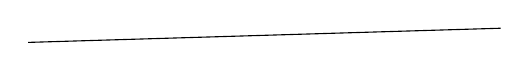
\begin{tikzpicture}\draw (0,0)--(6,.18);\end{tikzpicture}}
\[
Q^{2\nu+1}\qquad \xi:\ H^{\unsure{2i|i}}(Q^{2\nu+1})\text{---}
H^{2i+2}(Q^{2\nu\inserted{\text{\textcircled{$+1$}}}})(1)
\]
\margin{($0\leq i\leq2\nu$)}

\uline{bijectif} si $i\neq\nu$

injectif de conoyau $\mathbb Z/2\mathbb Z$ si $i=\nu$
\figure{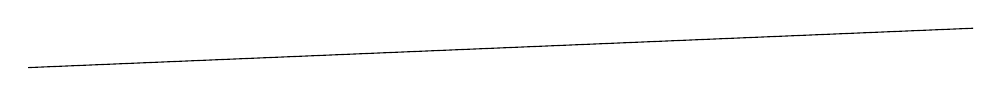
\begin{tikzpicture}\draw (0,0)--(12,.5);\end{tikzpicture}}
\mspage{31}
